\documentclass[a4paper, 12pt]{article}

\input{/home/nick/latex-preambles/xelatex.tex}

\setmainfont{Minion Pro}

\newcommand{\imagesPath}{.}

\title{
	\textbf{Εργαστήριο Δικτύων Υπολογιστών} \\~\\
	Εργαστηριακή Άσκηση 5 \\ 
	Στατική δρομολόγηση
}
\author{}
\date{}

\begin{document}
\maketitle
\begin{center}
	\begin{tabular}{|l|l|}
		\hline
		\textbf{Ονοματεπώνυμο:} Νικόλαος Παγώνας, el18175  & \textbf{Όνομα PC:} nick-ubuntu \\
		\hline
		\textbf{Ομάδα:} 1 (Τρίτη 10:45) & \textbf{Ημερομηνία Εξέτασης:} Τρίτη 29/03/2022 \\
		\hline
	\end{tabular}
\end{center}

\section*{Άσκηση 1: Δρομολόγηση σε ένα βήμα}

	\subsection*{1.1}
		Με τις εντολές:
		
		\begin{verbatim}
			PC1: 
			ifconfig em0 192.168.1.2/24
			
			PC2: 
			ifconfig em0 192.168.2.2/24
			
			R1: 
			ifconfig em0 192.168.1.1/24
			ifconfig em1 192.168.2.1/24
		\end{verbatim}

	\subsection*{1.2}
		Προσθέσαμε τη γραμμή:
		
		\begin{verbatim}
			gateway_enable="YES"
		\end{verbatim}

	\subsection*{1.3}
		Προσθέτουμε τη ζητούμενη εγγραφή με την εντολή:
		
		\begin{verbatim}
			route add –net 192.168.2.0/24 192.168.1.1
		\end{verbatim}

	\subsection*{1.4}
		Εκτελούμε \verb|netstat -rn|. Η σημαία "U" σημαίνει ότι η διαδρομή είναι ενεργή, η σημαία "G" σημαίνει ότι ο προορισμός είναι πύλη, που θα αποφασίσει για το πώς θα προωθήσει τα πακέτα περαιτέρω, ενώ η σημαία "S" σημαίνει ότι η διαδρομή έχει οριστεί στατικά.

	\subsection*{1.5}
		Δοκιμάζουμε \verb|ping 192.168.2.2| από το PC1 στο PC2 και παρατηρούμε ότι το PC1 δε λαμβάνει απάντηση.

	\subsection*{1.6}
		Με \verb|tcpdump -i em0| στα PC1 και PC2, παρατηρούμε ότι παράγονται πακέτα ICMP τόσο στο LAN1 όσο και στο LAN2. Παρολαυτά, στο PC2 δεν υπάρχει η κατάλληλη εγγραφή στον πίνακα δρομολόγησης ώστε να μπορεί να στείλει το PC2 ICMP reply στο PC1.

	\subsection*{1.7}
		Προσθέτουμε τη ζητούμενη εγγραφή με την εντολή:
		
		\begin{verbatim}
			route add -net 192.168.1.0/24 192.168.2.1
		\end{verbatim}

	\subsection*{1.8}
		Δοκιμάζουμε πάλι \verb|ping 192.168.2.2| από το PC1 στο PC2. Πλέον υπάρχει επικοινωνία.

	\subsection*{1.9}
		Δεν χρειάζεται να αλλάξουμε τον πίνακα δρομολόγησης του R1, διότι ο R1 διαθέτει διεπαφές και στα δύο υποδίκτυα (την \verb|em0| στο \verb|192.168.1.0/24| και την \verb|em1| στο \verb|192.168.2.0/24|), και άρα οι απαιτούμενες εγγραφές υπάρχουν ήδη στον πίνακα δρομολόγησής του.

\section*{Άσκηση 2: Proxy ARP}

	\subsection*{2.1}
		Καταργούμε τη στατική εγγραφή στο PC1 με την εντολή \verb|route del 192.168.2.0/24|.

	\subsection*{2.2}
		Αλλάζουμε το μήκος προθέματος στο PC1 με την εντολή \verb|ifconfig em0 192.168.1.2/20|.

	\subsection*{2.3}
		Από την προοπτική του PC1, τα PC2 και PC3 βρίσκονται στο ίδιο υποδίκτυο με αυτόν, αφού:
		
		\begin{verbatim} 
			PC1 IP & PC1 subnet mask = 192.168.1.2 & 255.255.240.0 = 192.168.0.0
			PC2 IP & PC1 subnet mask = 192.168.2.2 & 255.255.240.0 = 192.168.0.0
			PC3 IP & PC1 subnet mask = 192.168.2.3 & 255.255.240.0 = 192.168.0.0
		\end{verbatim}
	
	\subsection*{2.4} 
		Από το PC1 κάνουμε \verb|ping 192.168.2.2| και \verb|ping 192.168.2.3|. Και από τα δύο ping λαμβάνουμε "Host is down".

		Στον δρομολογητή ενεργοποιούμε το proxy ARP με την εντολή:
	
		\begin{verbatim}
			sysctl net.link.ether.inet.proxyall=1
		\end{verbatim}
		
	\subsection*{2.5}
		Επαναλαμβάνουμε το \verb|ping -c 1 192.168.2.2|. Τώρα το ping είναι επιτυχές. Αυτό συμβαίνει διότι ενεργοποιήσαμε τη λειτουργία proxy ARP στον R1, οπότε ο R1 απαντά στο ARP request του PC1 -που θέλει να μάθει τη φυσική διεύθυνση του PC2- με τη δική του διεύθυνση MAC, προωθεί το ICMP echo request στον PC2, απαντά πάλι με τη δική του διεύθυνση MAC στο ARP request του PC2 -που θέλει να μάθει τη φυσική διεύθυνση του PC1-, και τέλος προωθεί το ICMP echo reply του PC2 στο PC1.

	\subsection*{2.6}
		Επαναλαμβάνουμε το \verb|ping 192.168.2.3|. Το ping αποτυγχάνει, διότι δεν υπάρχει εγγραφή στον πίνακα δρομολόγησης του PC3 σχετική με το PC1, ώστε το PC3 να μπορεί να στείλει ICMP echo reply, όπως έγινε με το PC2.

	\subsection*{2.7}
		Προσθέτουμε τη στατική εγγραφή στο PC3 με την εντολή:
		
		\begin{verbatim}
			route add 192.168.1.0/24 192.168.2.1
		\end{verbatim}

	\subsection*{2.8}
		Καθαρίζουμε τους πίνακες ARP με την εντολή \verb|arp -d -a|.

	\subsection*{2.9}
		Ξεκινάμε τις ζητούμενες καταγραφές στο R1 με τις εντολές: 
		
		\begin{verbatim}
			tcpdump -e -i em0
			tcpdump -e -i em1
		\end{verbatim}
		
		Επαναλαμβάνουμε το προηγούμενο ping από το PC1 στο PC3: \verb|ping -c 1 192.168.2.3|.

	\subsection*{2.10}
		Παρατηρούμε ότι ο R1 απαντά στο ARP request του PC1 με τη δική του φυσική διεύθυνση, και συγκεκριμένα με τη φυσική διεύθυνση της διεπαφής του στο LAN1.

	\subsection*{2.11}
		Ο PC1 στέλνει το ICMP request προς τη διεύθυνση \verb|08:00:27:57:dd:d7|, δηλαδή τη φυσική διεύθυνση της διεπαφής του R1 στο LAN1.

	\subsection*{2.12}
		Ο PC3 λαμβάνει το ICMP request από τη φυσική διεύθυνση της διεπαφής του R1 στο LAN2.

	\subsection*{2.13} 
		\begin{figure}[H]
			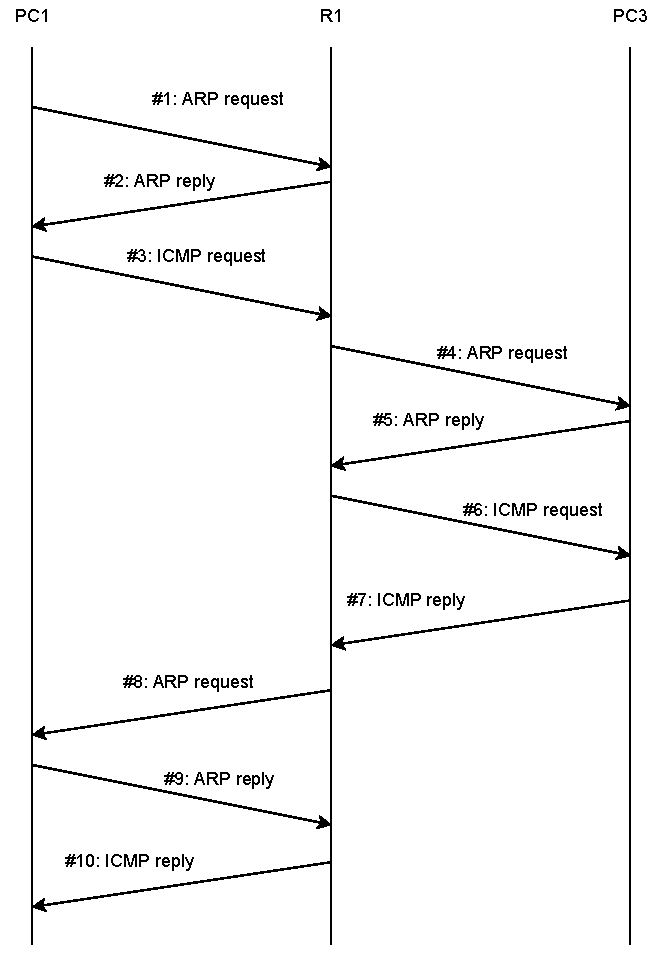
\includegraphics[width=0.75\linewidth]{\imagesPath/2.13.pdf}
		\end{figure}
		
		\begin{itemize}
			\item \#1: Επίλυση της φυσικής διεύθυνσης του PC3 για το PC1.
			\item \#2: Proxy ARP, απάντηση στο ARP request \#1. Ο R1 απαντά με τη δική του φυσική διεύθυνση αντί για τη διεύθυνση του PC3.
			\item \#3: ICMP request από το PC1 με προορισμό το PC3.
			\item \#4: Επίλυση της φυσικής διεύθυνσης του PC3 για το R1.
			\item \#5: Απάντηση του ARP reply \#4.
			\item \#6: Προώθηση του ICMP request \#3.
			\item \#7: Απάντηση του ICMP request \#6.
			\item \#8: Επίλυση της φυσικής διεύθυνσης του PC1 για το R1. Να σημειωθεί ότι ο R1 δεν γνωρίζει τη φυσική διεύθυνση του PC1 λόγω του ARP request \#1, αφού εκεί αναζητείται η φυσική διεύθυνση του PC3, και όχι του R1.
			\item \#9: Απάντηση του ARP request \#8.
			\item \#10: Προώθηση του ICMP reply \#7.
		\end{itemize}

	\subsection*{2.14}
		Ο πίνακας δρομολόγησης του PC1 (\verb|netstat -rn|) έχει εγγραφές για τη loopback, το υποδίκτυο \verb|192.168.0.0/20| και τη διεύθυνση \verb|192.168.1.2|. Από αυτές η μόνη που μπορεί να φανεί χρήσιμη είναι αυτή του υποδικτύου \verb|192.168.0.0/20|. Πρέπει λοιπόν το πρόθεμα δικτύου αυτής της εγγραφής να είναι τέτοιο ώστε να περιλαμβάνεται και το PC3 σε αυτό το υποδίκτυο. 
		
		\begin{verbatim}
			PC3 IPv4:           11000000.10101000.00000010.00000011
			PC1 subnet IPv4:    11000000.10101000.00000000.00000000
			max prefix match == 22 bits
		\end{verbatim}
		
		Επομένως το μέγιστο μήκος προθέματος για το PC1 είναι 22 bits.

	\subsection*{2.15}
		Δίνουμε στο PC1 την εντολή \verb|ifconfig em0 192.168.1.2/23|.

	\subsection*{2.16}
		Στο PC1 εκτελούμε: \verb|route add -net 192.168.2.0/24 -interface em0|

	\subsection*{2.17}
		Στον πίνακα δρομολόγησης του PC1 εμφανίζεται:
		
		\begin{verbatim}
			Destination       Gateway              Netif
			192.168.2.0/24    08:00:27:ca:53:74    em0
		\end{verbatim}

	\subsection*{2.18}
		Τώρα το ping προς τον PC3 είναι επιτυχές. Αυτό συμβαίνει διότι o PC1 βλέπει την εγγραφή \verb|192.168.2.0/24| στον πίνακα δρομολόγησης και στέλνει το πακέτο στον R1, ο οποίος το προωθεί στον PC3, και ο PC3 βλέπει την εγγραφή \verb|192.168.1.0| στον πίνακα δρομολόγησής του και μπορεί να απαντήσει. Για τα πακέτα ARP ισχύουν όσα έχουν αναφερθεί παραπάνω (proxy ARP κλπ).

	\subsection*{2.19}
		Στον R1 ακυρώνουμε το proxy ARP με την εντολή: \verb|sysctl net.link.ether.inet.proxyall=0|.

	\subsection*{2.20}
		Στο PC1 εκτελούμε: \verb|route change -net 192.168.2.0/24 192.168.1.1|.

	\subsection*{2.21}
		Στο PC1 εκτελούμε: \verb|ifconfig em0 192.168.1.2/24|.

	\subsection*{2.22} 
		Παρατηρούμε ότι η διαδρομή για το \verb|192.168.2.0/24| δεν υπάρχει πλέον στον πίνακα δρομολόγησης του PC1. Την επαναπροσδιορίζουμε με την εντολή \verb|route add -net 192.168.2.0/24 192.168.1.1|.

\section*{Άσκηση 3: Δρομολόγηση σε περισσότερα βήματα}

	\subsection*{3.1}
		Ορίζουμε διευθύνσεις IPv4 στον R1 με τις εντολές:
		
		\begin{verbatim}
			ifconfig em0 192.168.1.1/24
			ifconfig em1 172.17.17.1/30
		\end{verbatim}	

	\subsection*{3.2}
		Ορίζουμε διευθύνσεις IPv4 στον R2 με τις εντολές:
		
		\begin{verbatim}
			ifconfig em0 172.17.17.2/30
			ifconfig em1 192.168.2.1/24
		\end{verbatim}

	\subsection*{3.3}
		Εκτελούμε \verb|ping 192.168.2.2|. Εμφανίζεται μήνυμα "Destination Host Unreachable".

	\subsection*{3.4}
		Με \verb|tcpdump -e -i em0| και \verb|tcpdump -e -i em1| στον R1 ελέγχουμε τα πακέτα που εκπέμπονται στα LAN1 και WAN1 αντίστοιχα. Στο LAN1 παρατηρούμε μηνύματα "ICMP echo request" από το PC1 προς το R1, αλλά και μηνύματα "ICMP host 192.168.2.2 unreachable" από το R1 στο PC1. Στο WAN1 δεν παρατηρούνται μηνύματα ICMP, αφού ο R1 δεν γνωρίζει πού να προωθήσει τα πακέτα που προορίζονται για το PC2 (δεν διαθέτει σχετική εγγραφή στον πίνακα δρομολόγησης). 

	\subsection*{3.5}
		Από το PC1 εκτελούμε \verb|traceroute 192.168.2.2| και στην έξοδό της εντολής βλέπουμε 3 φορές το σύμβολο \verb|!H|, που σημαίνει ότι ο PC1 έλαβε μήνυμα "Destination host unreachable" από τον R1 (\verb|192.168.1.1|).

	\subsection*{3.6}
		Προσθέτουμε τη ζητούμενη εγγραφή μέσω της εντολής:
		
		\begin{verbatim}
			R1:
			route add -net 192.168.2.0/24 172.17.17.2
		\end{verbatim}


	\subsection*{3.7}
		Δοκιμάζουμε πάλι \verb|ping 192.168.2.2| από το PC1 στο PC2. Δεν εμφανίζεται πλέον "Destination Host Unreachable" αλλά πάλι δεν λαμβάνουμε απάντηση. 

	\subsection*{3.8}
		Με την εντολή \verb|tcpdump -i em0| στο PC2 βλέπουμε ότι στο LAN2 παράγονται μηνύματα:
		
		\begin{itemize}
			\item ICMP echo request: Έχει προκύψει από την προώθηση του ICMP echo request του PC1 από τον R2.
			\item ICMP echo reply: Έχει προκύψει ως απάντηση στο ICMP echo request από τον PC2.
			\item ICMP host 192.168.1.2 unreachable: Έχει προκύψει από τον R2 και προορίζεται για τον PC2, επειδή ο R2 δεν γνωρίζει πού να προωθήσει το ICMP echo reply του PC2 που προορίζεται για τον PC1 (δεν έχει εγγραφή στον πίνακα δρομολόγησης σχετική με το PC1).
		\end{itemize}

	\subsection*{3.9}
		Δοκιμάζουμε ξανά \verb|traceroute 192.168.2.2| από το PC1 προς το PC2. Δεν παρατηρούμε μηνύματα ICMP echo request στο WAN1 (εκτελέσαμε \verb|tcpdump -i em1| στο R1). Αντ' αυτού, παρατηρήσαμε UDP datagrams, επειδή η traceroute στέλνει UDP datagrams by default.

	\subsection*{3.10}
		Στο LAN2 (εκτελέσαμε \verb|tcpdump -i em1| στο R2) παρατηρούνται UDP datagrams και μηνύματα "ICMP 192.168.2.2 udp port 3344x unreachable", όπου $\text{x}=\{2,3,4,5\}$.

	\subsection*{3.11}
		Σύμφωνα με την ιστοσελίδα, δεν παράγεται το error message "ICMP host unreachable" ως απάντηση στο error message "ICMP 192.168.2.2 udp port 3344x unreachable", διότι εξ' ορισμού δεν παράγονται ICMP μηνύματα λάθους ως απάντηση σε άλλα ICMP μηνύματα λάθους (κάτι τέτοιο θα δημιουργούσε έναν κατακλυσμό από ICMP μηνύματα λάθους). 

	\subsection*{3.12}
		Στο R2 εκτελούμε την εντολή \verb|route add 192.168.1.0/24 172.17.17.1|.

	\subsection*{3.13}
		Πλέον μπορούμε να κάνουμε \verb|traceroute 192.168.2.2| από το PC1 στο PC2. Στο WAN1 (εκτελέσαμε \verb|tcpdump -i em1| στο R1) παράγονται μηνύματα "ICMP time exceeded in-transit", επειδή η traceroute ως γνωστόν στέλνει UDP datagrams με σταδιακά αυξανόμενο TTL (οπότε κάποια αναπόφευκτα θα αποκτήσουν TTL=0 όσο προωθούνται προς τον προορισμό) και "ICMP 192.168.2.2 udp port 3344x unreachable" (x $= \{2,3,4\}$), αφού δεν υπάρχει κάποια εφαρμογή που "ακούει" στις συγκεκριμένες πόρτες στο PC2.

	\subsection*{3.14}
		Κάνουμε \verb|ping 172.17.17.1| από το PC2. Παρατηρούμε ότι εμφανίζεται το μήνυμα "No route to host".

	\subsection*{3.15}
		Στο PC2 εκτελούμε \verb|route del 192.168.1.0/24|.

	\subsection*{3.16}
		Στο PC2 εκτελούμε \verb|route add default 192.168.2.1|.

	\subsection*{3.17}
		Στο PC2 εκτελούμε πάλι \verb|ping 172.17.17.1|. Το ping είναι επιτυχές αυτή τη φορά.
		
	\subsection*{3.18}
		Ο λόγος που το ping αρχικά δεν πετυχαίνει, ενώ στη συνέχεια πετυχαίνει, είναι επειδή την πρώτη φορά, στον πίνακα δρομολόγησης του PC2 δεν υπήρχε εγγραφή σχετική με τη διεύθυνση \verb|172.17.17.1|. Τη δεύτερη φορά όμως, επειδή προστίθεται εγγραφή για την προεπιλεγμένη πύλη, το ICMP request στέλνεται στη διεπαφή του R2 στο LAN2 και αυτός το προωθεί με επιτυχία στον προορισμό. 

\section*{Άσκηση 4: Ένα πιο πολύπλοκο δίκτυο με εναλλακτικές διαδρομές}

	\subsection*{4.1}
		Στο PC3 εκτελούμε:
		
		\begin{verbatim}
			ifconfig em0 up
			ifconfig em0 192.168.2.3/24
		\end{verbatim}

	\subsection*{4.2}
		Στο PC3 εκτελούμε:
		
		\begin{verbatim}
			route add -net 192.168.1.0/24 192.168.2.1
		\end{verbatim}

	\subsection*{4.3}
		Για το R1 έχουμε:
		
		\begin{verbatim}
			em0: LAN1
			ifconfig em0 192.168.1.1/24
			
			em1: WAN1
			ifconfig em1 172.17.17.1/30
			
			em2: WAN2
			ifconfig em2 172.17.17.5/30
		\end{verbatim}

	\subsection*{4.4}
		Για το R2 έχουμε:
		
		\begin{verbatim}
			em0: WAN1
			ifconfig em0 172.17.17.2/30
			
			em1: WAN3
			ifconfig em1 172.17.17.9/30
			
			em2: LAN2
			ifconfig em2 192.168.2.1/24
		\end{verbatim}

	\subsection*{4.5}
		Για το R3 έχουμε:
		
		\begin{verbatim}
			em0: WAN2
			ifconfig em0 172.17.17.6/30
			
			em1: WAN3
			ifconfig em1 172.17.17.10/30
		\end{verbatim}

	\subsection*{4.6}
		Στον R1 εκτελούμε:
		
		\begin{verbatim}
			route add -net 192.168.2.0/24 172.17.17.2
		\end{verbatim}

	\subsection*{4.7}
		Στον R2 εκτελούμε:
		
		\begin{verbatim}
			route add -net 192.168.1.0/24 172.17.17.1
		\end{verbatim}

	\subsection*{4.8}
		Στον R3 εκτελούμε:

		\begin{verbatim}
			route add -net 192.168.1.0/24 172.17.17.5
			route add -net 192.168.2.0/24 172.17.17.9
		\end{verbatim}
	
	\subsection*{4.9}
		Στον R1 εκτελούμε:
		
		\begin{verbatim}
			route add -host 192.168.2.3 172.17.17.6
		\end{verbatim}
		
		Εκτελούμε \verb|netstat -rn|. Η σημαία που δηλώνει ότι πρόκειται για υπολογιστή είναι η "H".

	\subsection*{4.10}
		Δοκιμάζουμε \verb|traceroute 192.168.2.2| από το PC1 στο PC2. Βλέπουμε 3 βήματα.

	\subsection*{4.11}
		Δοκιμάζουμε \verb|ping -c 1 192.168.2.2| από το PC1 στο PC2. Το ICMP reply έχει TTL = 62, οπότε με βάση αυτή την τιμή βλέπουμε 3 βήματα, αφού:

		\begin{itemize}
			\item PC2: το πακέτο φεύγει με TTL = 64
			\item 1ος δρομολογητής, 1ο βήμα: μειώνει το TTL κατά 1, και το πακέτο φεύγει με TTL = 63
			\item 2ος δρομολογητής, 2ο βήμα: μειώνει το TTL κατά 1, και το πακέτο φεύγει με TTL = 62
			\item PC1, 3ο βήμα: το πακέτο φτάνει έχοντας TTL = 62.
		\end{itemize}
		
	\subsection*{4.12}
		Δοκιμάζουμε \verb|traceroute 192.168.2.3| από το PC1 στο PC3. Βλέπουμε 4 βήματα.

	\subsection*{4.13}
		Δοκιμάζουμε \verb|ping -c 1 192.168.2.3| από το PC1 στο PC3. Το ICMP reply έχει TTL = 62, οπότε με βάση την τιμή αυτή βλέπουμε 3 βήματα. Η αιτιολόγηση είναι ίδια με αυτή του ερωτήματος 4.11.

	\subsection*{4.14}
		Με βάση την έξοδο της εντολής traceroute, το ICMP echo request προς το PC3 ακολουθεί τη διαδρομή:
		
		\begin{verbatim}
			PC1 --> R1 --> R3 --> R2 --> PC3
		\end{verbatim}

	\subsection*{4.15}
		Το ICMP echo reply προς το PC1 ακολουθεί τη διαδρομή:
		
		\begin{verbatim}
			PC3 --> R2 --> R1 --> PC1
		\end{verbatim}
		
		Η διαφορά των δύο διαδρομών έγκειται στο ότι στην περίπτωση του ερωτήματος 4.14, ο R1 έχει δύο εγγραφές σχετικές με το PC3 στον πίνακα δρομολόγησης, μία που αναφέρεται στη διεύθυνση του PC3 και μόνο, και μία που αναφέρεται στο LAN2. Από τις δύο, ο R1 επιλέγει το ταίριασμα μέγιστου προθέματος, δηλαδή την εγγραφή που αναφέρεται στη διεύθυνση του PC3, και με βάση αυτή την εγγραφή προωθεί το πακέτο στον R3. Αντίθετα, στον πίνακα δρομολόγησης του R2 βρίσκεται η στατική εγγραφή που προσθέσαμε προηγουμένως, ώστε ο R2 να προωθεί πακέτα για το LAN1 μέσω του R1, η οποία είναι και η μόνη έγκυρη εγγραφή, οπότε είναι και αυτή που επιλέγεται.

	\subsection*{4.16}
		Απενεργοποιούμε την διεπαφή του R1 στο WAN1 και ξεκινάμε τη ζητούμενη καταγραφή στο R2 με την εντολή \verb|tcpdump -i em2|.

	\subsection*{4.17}
		Δοκιμάζουμε \verb|traceroute 192.168.2.2| από το PC1 στο PC2 και αφήνουμε να ολοκληρωθούν τουλάχιστον 3 βήματα. Δεν παρατηρούμε να φτάνουν ή να παράγονται πακέτα UDP στο PC2. 

	\subsection*{4.18}
		Δοκιμάζουμε \verb|traceroute 192.168.2.3| από το PC1 στο PC3 και αφήνουμε να ολοκληρωθούν τουλάχιστον 4 βήματα. Παρατηρούμε ότι φτάνουν και παράγονται πακέτα UDP στο PC3. 
		
	\subsection*{4.19}
		Η ζητούμενη σύνταξη της εντολής \verb|route| είναι:
		
		\begin{verbatim}
			R1:
			route change -net 192.168.2.0/24 172.17.17.6
			
			R2:
			route change -net 192.168.1.0/24 172.17.17.10
		\end{verbatim}
		
		Με χρήση της traceroute επιβεβαιώνουμε ότι υπάρχει επικοινωνία μετά την αλλαγή.
		
	\subsection*{4.20}
		Στον R1 εκτελούμε \verb|route show 192.168.2.2| και \verb|route show 192.168.2.3|. Παρατηρούμε ότι στην πρώτη περίπτωση το πεδίο "destination" αναφέρεται στο υποδίκτυο LAN2 -γι' αυτόν τον λόγο υπάρχει και η επιπλέον πληροφορία για τη μάσκα υποδικτύου-, ενώ στην δεύτερη περίπτωση το πεδίο "destination" αναφέρεται συγκεκριμένα στον host PC3 -γι' αυτόν τον λόγο υπάρχει και η επιπλέον σημαία "HOST". 

	\subsection*{4.21}
		Επιλέγεται η εγγραφή που αναφέρεται στον host \verb|192.168.2.3| (πεδίο destination: \verb|192.168.2.3|), επειδή αυτή η εγγραφή προσφέρει το μέγιστο ταίριασμα προθέματος.

\section*{Άσκηση 5: Βρόχοι κατά τη δρομολόγηση}

	\subsection*{5.1}
		Τροποποιούμε τη ζητούμενη εγγραφή στον R3 με την εντολή:
		
		\begin{verbatim}
			route change -net 192.168.2.0/24 172.17.17.5
		\end{verbatim}

	\subsection*{5.2}
		Εκτελούμε \verb|ping -c 1 192.168.2.2| από το PC1 στο PC2. Tο ping δεν είναι επιτυχές, καθώς εμφανίζεται μήνυμα "Time to live exceeded".

	\subsection*{5.3} 
		Το μήνυμα λάθους προέρχεται από τη διεπαφή του R3 στο WAN2, με διεύθυνση \verb|172.17.17.6|. 

	\subsection*{5.4} 
		Πρέπει να καταγράψουμε στον R1 και στο δίκτυο WAN2, επειδή εκεί έχει δημιουργηθεί ο βρόχος λόγω της στατικής εγγραφής που τροποποιήσαμε στο ερώτημα 5.1. 

	\subsection*{5.5} 
		Πρέπει να εφαρμόσουμε το φίλτρο \verb|"icmp[icmptype] == icmp-echo"|.

	\subsection*{5.6} 
		Ξεκινάμε στον R1 την καταγραφή που περιγράφηκε παραπάνω με την εντολή:
		
		\begin{verbatim}
			tcpdump -e -i em2 "icmp[icmptype] == icmp-echo"
		\end{verbatim} 
		
		Παρατηρούμε ότι λήφθηκαν 64 πακέτα, ενώ καταγράφηκαν 63 πακέτα. Το ένα πακέτο που λήφθηκε αλλά δεν καταγράφηκε είναι τύπου ICMP time exceeded in-transit. Έτσι έχουμε ότι εμφανίσθηκαν στο WAN2 63 πακέτα ICMP echo request. Τέλος, από το PC1 παράχθηκε μόνο ένα πακέτο ICMP echo request, όπως εξάλλου ορίσαμε και στην εντολή ping με την παράμετρο \verb|-c 1|. 

	\subsection*{5.7} 
		Ξεκινάμε τη ζητούμενη καταγραφή στο R1 με την εντολή \verb+tcpdump -l -i em0 | tee capture1+. Αντίστοιχα στο R3 με την εντολή \verb+tcpdump -l -i em0 | tee capture2+.

	\subsection*{5.8} 
		Εκτελούμε \verb|traceroute -I -q 1 192.168.2.2| από το PC1 στο PC2. Εμφανίζονται 64 βήματα μέχρι να ολοκληρωθεί η εκτέλεση της εντολής. Η διαδρομή που καταγράφουμε είναι η:
		
		\begin{verbatim}
			PC1 --> R1 --> R3 --> R1 --> R3 --> ... --> R1 --> R3
		\end{verbatim}
		
		δηλαδή ο βρόχος που έχει σχηματιστεί.

	\subsection*{5.9} 
		Σταματάμε τις καταγραφές. Με την εντολή \verb+grep "ICMP echo request" capture1 | wc -l+ στο R1 βρίσκουμε ότι στάλθηκαν 64 πακέτα ICMP echo request από το PC1. 

	\subsection*{5.10} 
		Με την εντολή \verb+grep "ICMP echo request" capture2 | wc -l+ στο R3 βρίσκουμε ότι εμφανίστηκαν 2016 πακέτα ICMP echo request στο WAN2. \\
		
		Η εξήγηση είναι η εξής: \\
		
		Έστω ότι από το PC1 ξεκινάει ένα πακέτο με $\text{TTL} = T$. Αυτό θα σταλεί στον R1, και εκεί θα αποκτήσει $\text{TTL} = T-1$. Ύστερα, θα μπει στον βρόχο R1 $\rightarrow$ R3 $\rightarrow$ R1..., μέχρι το TTL του να μηδενιστεί, οπότε και θα απορριφθεί από τον αντίστοιχο δρομολογητή. Επομένως, ένα πακέτο με $\text{TTL} = T$, θα εμφανιστεί συνολικά $T-1$ φορές στο WAN2. Επειδή η εντολή traceroute στέλνει ένα πακέτο ανά βήμα (παράμετρος \verb|-q 1|), και σε κάθε βήμα το TTL αυξάνεται κατά 1, ο συνολικός αριθμός πακέτων ICMP echo request που θα εμφανιστούν στο WAN2 είναι:
		
		\[
			1 + 2 + 3 + ... + 63 = \frac{63\cdot(63+1)}{2} = 2016 \text{ πακέτα}.
		\]

	\subsection*{5.11} 
		Με την εντολή \verb+grep "ICMP time exceeded in-transit" capture2 | wc -l+ βρίσκουμε ότι εμφανίστηκαν 32 πακέτα ICMP time exceeded στο WAN2. Αυτό συμβαίνει διότι από τα 64 πακέτα ICMP echo request που παράχθηκαν συνολικά από το PC1, τα μισά θα απορριφθούν από τον R1 (αυτά με αρχικό $\text{TTL} = 1,3,5,7,...,63$), οπότε θα σταλεί μήνυμα ICMP time exceeded από τον R1 στο PC1 μέσω του LAN1, ενώ τα άλλα μισά θα απορριφθούν από τον R2 (αυτά με αρχικό $\text{TTL} = 2,4,6,8,...,64$), οπότε θα σταλεί μήνυμα ICMP time exceeded από τον R2 στον R1 μέσω του WAN2. Επομένως, τα 32 μηνύματα ICMP time exceeded που καταγράφηκαν αφορούν τα μηνύματα ICMP echo request με αρχικό TTL άρτιο. 

	\subsection*{5.12} 
		Μπορούμε να αποφύγουμε την αποθήκευση σε αρχείο ως εξής:
		
		\begin{verbatim}
			Question 5.9:
			R1: tcpdump -i em0 "icmp[icmptype] == icmp-echo"
			
			Question 5.10:
			R3: tcpdump -i em0 "icmp[icmptype] == icmp-echo"
			
			Question 5.11:
			R3: tcpdump -i em0 "icmp[icmptype] == icmp-timexceed"
		\end{verbatim}
		
		Σε κάθε περίπτωση η απάντηση που ψάχνουμε δίνεται αφού τερματίσουμε την εντολή tcpdump με Ctrl-C, στη γραμμή \verb|"xxxx packets captured"|.

	\subsection*{5.13} 
		Τα πακέτα ICMP echo request που παράχθηκαν από την εντολή ping έχουν μήκος 64 bytes και αρχικό TTL = 64, ενώ τα πακέτα ICMP echo request που παράχθηκαν από την εντολή traceroute έχουν μήκος 28 bytes και αρχικό TTL που κυμαίνεται από 1 έως 64. 

	\subsection*{5.14} 
		Τα πακέτα ICMP echo request δεν κυκλοφορούν αενάως στο δίκτυο, διότι κάθε φορά που το πακέτο περνά από έναν δρομολογητή, αυτός μειώνει το TTL του κατά 1, και όταν το TTL γίνει μηδέν, τότε ο δρομολογητής απορρίπτει το πακέτο και στέλνει μήνυμα ICMP time exceeded. 

\section*{Άσκηση 6: Χωρισμός σε υποδίκτυα}

	\subsection*{6.1}
		LAN1, $120$ υπολογιστές, πρέπει: 
		
		\[
			2^n-2>120 \implies n = 7 \implies \text{Μήκος προθέματος LAN1} = 32 - 7 = 25. 
		\]
		
		Λαμβάνουμε υπόψιν μας το γεγονός ότι το μπλοκ διευθύνσεων 172.17.17.129-172.17.17.138 είναι δεσμευμένο από τους δρομολογητές.
		
		\begin{verbatim}
			129 dec = 1000 0001 bin
			138 dec = 1000 1010 bin
		\end{verbatim}
		
		βλέπουμε ότι μπορούμε να διαθέσουμε το μπλοκ 172.17.17.0-172.17.17.127, επομένως η διεύθυνση υποδικτύου του LAN1 είναι \textbf{172.17.17.0/25}.

	\subsection*{6.2}
		LAN2, $60$ υπολογιστές, πρέπει:
		\[ 
			2^n-2>60 \implies n = 6 \implies \text{Μήκος προθέματος LAN2} = 32 - 6 = 26. 
		\]
		
		βλέπουμε ότι μπορούμε να διαθέσουμε το μπλοκ 172.17.17.192-172.17.17.255, επομένως η διεύθυνση υποδικτύου του LAN2 είναι \textbf{172.17.17.192/26}.

	\subsection*{6.3}
		LAN3, $30$ υπολογιστές, πρέπει: 
		
		\[
			2^n-2>30 \implies n = 5 \implies \text{Μήκος προθέματος LAN3} = 32 - 5 = 27. 
		\]
		
		βλέπουμε ότι μπορούμε να διαθέσουμε το μπλοκ 172.17.17.160-172.17.17.191, επομένως η διεύθυνση υποδικτύου του LAN3 είναι \textbf{172.17.17.160/27}.

	\subsection*{6.4}
		Στο PC1 εκτελούμε: 
		
		\begin{verbatim}
			ifconfig em0 172.17.17.1/25
		\end{verbatim}
		
		Eνώ στον R1 εκτελούμε:
		
		\begin{verbatim}
			ifconfig em0 172.17.17.126/25
		\end{verbatim}
		
	\subsection*{6.5}
		Στο PC4 εκτελούμε:
		
		\begin{verbatim}
			ifconfig em0 172.17.17.161/27
		\end{verbatim}
		
		Eνώ στον R3 εκτελούμε:
		
		\begin{verbatim}
			ifconfig em0 172.17.17.190/27
		\end{verbatim}

	\subsection*{6.6}
		Στον R2 εκτελούμε:
		
		\begin{verbatim}
			ifconfig em2 172.17.17.193/26
		\end{verbatim}
		
		Στο PC2 εκτελούμε:
		
		\begin{verbatim}
			ifconfig em0 172.17.17.253/26
		\end{verbatim}
		
		Ενώ στο PC3 εκτελούμε:
		
		\begin{verbatim}
			ifconfig em0 172.17.17.254/26
		\end{verbatim}

	\subsection*{6.7}
		Εκτελούμε τις εντολές:
		
		\begin{verbatim}
			PC1: route add default 172.17.17.126
			PC2: route add default 172.17.17.193
			PC3: route add default 172.17.17.193
			PC4: route add default 172.17.17.190
		\end{verbatim}

	\subsection*{6.8}
		Στον R1 εκτελούμε:
		
		\begin{verbatim}
			route add -net 172.17.17.192/26 172.17.17.130
			route add -net 172.17.17.160/27 172.17.17.130
		\end{verbatim}

	\subsection*{6.9}
		Στον R2 εκτελούμε:
		
		\begin{verbatim}
			route add -net 172.17.17.0/25 172.17.17.137
			route add -net 172.17.17.160/27 172.17.17.137
		\end{verbatim}

	\subsection*{6.10}
		Στον R3 εκτελούμε:
		
		\begin{verbatim}
			route add -net 172.17.17.0/25 172.17.17.133
			route add -net 172.17.17.192/26 172.17.17.133
		\end{verbatim}

	\subsection*{6.11}
		Για να επιβεβαιώσουμε ότι υπάρχει επικοινωνία ανάμεσα σε όλα τα LAN, εκτελούμε:
		
		\begin{verbatim}
			PC1: ping -c 1 172.17.17.253
			PC2: ping -c 1 172.17.17.161
			PC3: ping -c 1 172.17.17.1
		\end{verbatim}
		
		Και τα τρία ping είναι επιτυχή.

\section*{Άσκηση 7: Ταυτόσημες διευθύνσεις IP}

	Επιβεβαιώνουμε ότι τα PC1, PC2 και PC3 επικοινωνούν μεταξύ τους εκτελώντας:
	
	\begin{verbatim}
		PC1 <-> PC2: ping -c 1 172.17.17.253
		PC1 <-> PC3: ping -c 1 172.17.17.254
		PC2 <-> PC3: ping -c 1 172.17.17.254
	\end{verbatim}
	
	\subsection*{7.1}
		Με \verb|ifconfig em0| στα PC2,3 βρίσκουμε ότι:
		
		\begin{verbatim}
			PC2 MAC address == 08:00:27:10:0c:23
			PC3 MAC address == 08:00:27:be:32:ef
		\end{verbatim}

	\subsection*{7.2}
		Στο PC2 εκτελούμε \verb|ifconfig em0 172.17.17.254/26|.

	\subsection*{7.3}
		Εμφανίστηκε στο PC2 η ένδειξη:
		
		\begin{verbatim}
			PC kernel: arp: 08:00:27:be:32:ef is using my IP address 172.17.17.254 on em0!
		\end{verbatim}

	\subsection*{7.4}
		Ναι, εμφανίστηκε στο PC3 η ένδειξη:
		
		\begin{verbatim}
			PC kernel: arp: 08:00:27:10:0c:23 is using my IP address 172.17.17.254 on em0!
		\end{verbatim}

	\subsection*{7.5}
		Ναι, με \verb|ifconfig em0| στο PC2 βλέπουμε ότι η IP διεύθυνση έχει οριστεί κανονικά. Το νόημα των μηνυμάτων λάθους είναι απλώς να ενημερώσει τους χρήστες των δύο μηχανημάτων ότι μοιράζονται την ίδια διεύθυνση IPv4.

	\subsection*{7.6}
		Όχι, ο R2 δεν παραμένει ως προεπιλεγμένη πύλη στο PC2 (\verb|netstat -rn|), επειδή εκτελέσαμε \verb|ifconfig| και αλλάξαμε την IP διεύθυνση του PC2. Όταν γίνεται αυτό, η προεπιλεγμένη πύλη διαγράφεται από τον πίνακα δρομολόγησης.

	\subsection*{7.7}
		Στο PC2 ορίζουμε και πάλι ως προεπιλεγμένη πύλη τον δρομολογητή R2 με την εντολή: 
		
		\begin{verbatim}
			route add default 172.17.17.193
		\end{verbatim}

	\subsection*{7.8}
		Καθαρίζουμε τους πίνακες ARP στα PC2, PC3 και R2 με την εντολή \verb|arp -d -a|.

	\subsection*{7.9}
		Ξεκινάμε τη ζητούμενη καταγραφή στον R2 με την εντολή \verb|tcpdump -i em2 "arp"|.

	\subsection*{7.10}
		Ξεκινάμε τις ζητούμενες καταγραφές εκτελώντας την εντολή \verb|tcpdump -n -i em0 "tcp"| στα PC2 και PC3.

	\subsection*{7.11}
		Από το PC1 εκτελούμε \verb|ssh lab@172.17.17.254|. Εμφανίζεται ένδειξη λάθους:
		
		\begin{verbatim}
			ssh_exchange_identification: read: Connection reset by peer
		\end{verbatim}

	\subsection*{7.12}
		Σταματάμε τις καταγραφές και επαναλαμβάνουμε το \verb|ssh lab@172.17.17.254|. Αυτή τη φορά η προσπάθεια είναι επιτυχής.

	\subsection*{7.13}
		Με την εντολή \verb|arp -a| στον R2 καταγράφουμε:
		
		\begin{verbatim}
			PC2: 172.17.17.254 at 08:00:27:10:0c:23 on em2
		\end{verbatim}
		
		Δεν υπάρχει εγγραφή για το PC3.

	\subsection*{7.14}
		Στην καταγραφή πακέτων arp, το PC3 απάντησε πρώτο στο ARP Request του R2, ενώ το PC2 απάντησε δεύτερο. 

	\subsection*{7.15}
		Η διεύθυνση MAC που περιέχει ο πίνακας ARP του R2 ανήκει στο PC2.

	\subsection*{7.16}
		Την δεύτερη φορά συνδεθήκαμε στο PC2, επειδή το PC2 απάντησε δεύτερο και έτσι η πιο πρόσφατη εγγραφή στον πίνακα ARP έδειχνε ότι η κοινή IPv4 διεύθυνση αντιστοιχεί στην φυσική διεύθυνση του PC2.

	\subsection*{7.17}
		Άλλοι τρόποι με τους οποίους μπορούμε να καταλάβουμε σε ποιο μηχάνημα έχουμε συνδεθεί, πέρα από τον τρόπο που χρησιμοποιήσαμε παραπάνω (δηλαδή μέσω της καταγραφής των πακέτων arp):
		
		\begin{itemize}
			\item Μπορούμε να εκτελέσουμε \verb|ifconfig em0| και να δούμε τη διεύθυνση MAC που αναγράφεται στην έξοδο της εντολής.
			\item Μπορούμε να εκτελέσουμε την εντολή \verb|w| στα PC2, PC3. Στο ένα από τα δύο θα υπάρχει μόνο ο χρήστης \verb|root|, ενώ στο άλλο θα φαίνεται ότι έχει συνδεθεί και ένας χρήστης \verb|lab|.
			\item Μππορούμε να εκτελέσουμε την εντολή \verb+netstat | grep ssh+ στα PC2, PC3. Στο ένα από τα δύο θα υπάρχει μια σύνδεση ssh που θα περιλαμβάνει τη διεύθυνση IPv4 του PC1 και τη διεύθυνση IPv4 του μηχανήματος που έχει γίνει η σύνδεση.
		\end{itemize}

	\subsection*{7.18} 
		Στον R2 λήφθηκε πρώτα το ARP reply από το PC3 και ύστερα από το PC2. Στις δύο καταγραφές TCP τεμαχίων παρατηρούμε ότι τα τεμάχια έχουν τις εξής σημαίες:
		
		\begin{itemize}
			\item Καταγραφή PC3:
				\begin{itemize}
					\item SYN: από το PC1 στο PC3, με σκοπό να ξεκινήσει η τριπλή χειραψία
					\item SYN, ACK: η απάντηση του PC3 προς το PC1, το δεύτερο τεμάχιο της χειραψίας
					\item SYN, ACK: επανάληψη του παραπάνω
					\item SYN, ACK: επανάληψη του παραπάνω
					\item SYN, ACK: επανάληψη του παραπάνω, τελικά εγκαταλείπεται η προσπάθεια, αφού δεν λαμβάνεται ποτέ το πακέτο με σημαία ACK (τρίτο τεμάχιο της χειραψίας)
				\end{itemize}
			\item Καταγραφή PC2 (πλέον ο R2 έχει λάβει ARP reply από το PC2, και έτσι τα επόμενα TCP τεμάχια με προορισμό τη διεύθυνση 172.17.17.254 στέλνονται στο PC2, και γι' αυτό δημιουργείται η "σύγχυση" που προκαλεί την αποτυχία του πρώτου SSH): 
				\begin{itemize}
					\item ACK: από το PC1 στο PC2, είναι το τρίτο τεμάχιο της χειραψίας που δεν πάει ποτέ στο PC3, που έστειλε το δεύτερο τεμάχιο της χειραψίας
					\item RST: από το PC2 στο PC1, αφού ο PC2 δεν έχει εγκατεστημένη κάποια σύνδεση με το PC1 και έτσι στέλνει τεμάχιο με σκοπό τον τερματισμό της παραπάνω επικοινωνίας.
					\item PSH, ACK: από το PC1 στο PC3, δείχνει ότι τα δεδομένα πρέπει να προωθηθούν στην εφαρμογή
					\item RST: από το PC2 στο PC1 με σκοπό τον τερματισμό της σύνδεσης
					\item RST: από το PC1 στο PC2 με σκοπό τον τερματισμό της σύνδεσης
					\item RST: από το PC1 στο PC2 με σκοπό τον τερματισμό της σύνδεσης
					\item RST: από το PC1 στο PC2 με σκοπό τον τερματισμό της σύνδεσης
				\end{itemize}
		\end{itemize} 
		
		Αυτή η "σύγχυση" επιλύεται τη δεύτερη φορά που συνδεόμαστε με SSH, αφού πλέον υπάρχει η εγγραφή στον πίνακα ARP του R2 που αντιστοιχεί την IPv4 διεύθυνση 172.17.17.254 με την MAC διεύθυνση του PC2, και η σύνδεση με SSH μεταξύ PC1 και PC2 είναι επιτυχής.
	
\end{document}